\documentclass[10pt,a4paper]{article}
\usepackage[utf8]{inputenc}
\usepackage{fancyhdr}
\usepackage{ngerman}
\usepackage{floatflt}
\usepackage{float}
\usepackage{graphicx}
\usepackage{tabularx}
\usepackage[ampersand]{easylist} % Aufzählung mit &
\usepackage{amsmath}
\usepackage{amsfonts}
\usepackage{amssymb}
\usepackage{array}
\usepackage{framed}
\usepackage[hidelinks]{hyperref}
\usepackage[left=3.5cm,right=2cm,top=2cm,bottom=2cm,includeheadfoot]{geometry}
\reversemarginpar
\pagestyle{fancy} %eigener Seitenstil
\setlength{\parindent}{0pt}

%Formatierung der Tabellen
\usepackage[table]{xcolor}
\renewcommand{\arraystretch}{1.3} % Zeilenabstand für Tabellen
\setlength\arrayrulewidth{0.7pt}

\usepackage{color}

%Farben für die Syntaxhervorhebung
\definecolor{pblue}{rgb}{0.13,0.13,1}
\definecolor{pgreen}{rgb}{0,0.5,0}
\definecolor{pred}{rgb}{0.9,0,0}
\definecolor{pgrey}{rgb}{0.46,0.45,0.48}

% Pakete für die Code-Formatierung von Programmcode
\usepackage{todonotes}
\usepackage{listings}
\newcommand\fnurl[2]{\href{#1}{#2}\footnote{\url{#1}}}

\renewcommand{\ttdefault}{pcr}
\lstdefinelanguage{pseudo}{
  morekeywords={if, then, else, for, in, remove, from, case, do, forever, to, return, False, True, Algorithm, Input, Output},
  literate={<=} {$\le$}{2} {!=} {$\neq$}{2} {=} {$\leftarrow$}{2} {==} {=}{2} {&&} {$\cap$}{2} {||} {$\cup$}{2},
  commentstyle=\textit,
  keywordstyle=\bfseries,
  sensitive=true,%
  morecomment=[s]{\{}{\}},%
  morestring=[b]',%
}
\lstset{language=Java,
  numbers=left,
  frame=none,
  showspaces=false,
  showtabs=false,
  breaklines=true,
  showstringspaces=false,
  breakatwhitespace=true,
  commentstyle=\color{pgreen},
  keywordstyle=\color{pblue},
  stringstyle=\color{pred},
  basicstyle=\ttfamily,
  moredelim=[il][\textcolor{pgrey}]{!!},
  moredelim=[is][\textcolor{pgrey}]{\%\%}{\%\%}
}

\lstset{literate=
  {á}{{\'a}}1 {é}{{\'e}}1 {í}{{\'i}}1 {ó}{{\'o}}1 {ú}{{\'u}}1
  {Á}{{\'A}}1 {É}{{\'E}}1 {Í}{{\'I}}1 {Ó}{{\'O}}1 {Ú}{{\'U}}1
  {à}{{\`a}}1 {è}{{\`e}}1 {ì}{{\`i}}1 {ò}{{\`o}}1 {ù}{{\`u}}1
  {À}{{\`A}}1 {È}{{\'E}}1 {Ì}{{\`I}}1 {Ò}{{\`O}}1 {Ù}{{\`U}}1
  {ä}{{\"a}}1 {ë}{{\"e}}1 {ï}{{\"i}}1 {ö}{{\"o}}1 {ü}{{\"u}}1
  {Ä}{{\"A}}1 {Ë}{{\"E}}1 {Ï}{{\"I}}1 {Ö}{{\"O}}1 {Ü}{{\"U}}1
  {â}{{\^a}}1 {ê}{{\^e}}1 {î}{{\^i}}1 {ô}{{\^o}}1 {û}{{\^u}}1
  {Â}{{\^A}}1 {Ê}{{\^E}}1 {Î}{{\^I}}1 {Ô}{{\^O}}1 {Û}{{\^U}}1
  {œ}{{\oe}}1 {Œ}{{\OE}}1 {æ}{{\ae}}1 {Æ}{{\AE}}1 {ß}{{\ss}}1
  {ç}{{\c c}}1 {Ç}{{\c C}}1 {ø}{{\o}}1 {å}{{\r a}}1 {Å}{{\r A}}1
  {€}{{\EUR}}1 {£}{{\pounds}}1
}

\makeatletter
\let\ps@plain\ps@fancy 
\makeatother

\title{InfSi3 Zusammenfassung}

\author{
	Roman Ehrbar\\
	\and
	Oliver Nietlispach\\
	\and
	Samuel Jost\\
	\and
	Etienne Georgy
	}

\date{\today}

\begin{document}
\maketitle
\tableofcontents
\listoftodos
\newpage 

\section{Einleitung}

\subsection{Information Security Management}
Kleiner Rückblick zu den Begriffen aus InfSi1:
\begin{description}
	\item[Asset] Wert aus Sicht der Organisation, ob materiell oder immateriell, Informationen oder Dienstleistungen.
	\item[Threat] Bedrohung, möglicher Grund für einen ungewollten Vorfall, der das System oder die Organisation schädigen kann.
	\item[Vulnerabilities] Schwachstelle einer Schutzmassnahme, die durch eine oder mehrere Bedrohungen ausgenutzt werden kann.
	\item[Controls] Gegenmassnahme als Mittel zur Risikohandhabung.
	\item[Gefährdung] Zusammenspiel von Asset, Threat und Vulnerabilities.
	\item[Applied Threat] Die Gefährdung ist eine Bedrohung, die konkret über eine Schwachstelle auf ein Objekt einwirkt. (Bedrohung und Schaden)
	\item[Risiko] = Wahrscheinlichkeit eines Zwischenfalls * Schaden = Bedrohung * Verletzlichkeit * Schaden
\end{description}

\subsection{Treiber für Informationssicherheit}
Als hauptsächliche Treiber der Informationssicherheit zählt die \textbf{Konformität zu Gesetz und Vorschriften}.

Folgendes liefert ein Teil von Gesetzen und Vorschriften in den verschiedenen Sparten:
\begin{easylist}[itemize]
	& Bearbeiter von Personendaten
	&& Diverse Strafgesetzbuch Artikel
	&& Datenschutzgesetz (DSG)
	&& US Health Insurance Portability and Accountability Act (HIPAA)
	& Finanzdienstleister
	&& Bankgesetze (Bankgeheimnis, etc.)
	&& EU Directive on Payment Services (PSD)
	&& Payment Card Industry Data Security Standard (PCI)
	& Telecom/ICT-Anbieter
	&& Fernmeldegesetz
	&& Lawful Interception
	& Allgemeines Controlling
	&& Sarbanes-Oxley Act (SOX), US-börsenkotierte Firmen
\end{easylist} 

\todo[inline]{Gesetzliche Anforderungen}
\todo[inline]{Bedrohungen}

\section{Secure Software / Software Security}

Durch das Aufkommen des Internets nahm auch die vom \textit{National Institute of Standards and Technology} (NIST) erfassten Vulnerabilities mit hohem Ausmass zu.

\subsection{Most Dangerous Software Errors}
Die 25 häufigsten Schwachstellen können in drei Kategorien eingeteilt werden:
\begin{itemize}
	\item Ausgelöst durch unsichere Wege, in denen die Daten gesendet und empfangen werden. Dazu zählen \textit{SQL Injection}, \textit{OS Command Injection}, \textit{XSS}, \textit{CSRF} und \textit{Open Redirect}.
	\item Ausgelöst durch die unsichere Handhabung von Systemressourcen. Dazu gehören \textit{Classic Buffer Overflow}, \textit{Path Traversal}, \textit{Uncontrolled Format String}, \textit{Potentially Dangerous Function} und \textit{Integer Overflow}.
	\item Ausgelöst durch falsche Verwendung, Missbrauch oder Ignorierung von defensiven Sicherheitsmechanismen. Dazu zählen \textit{Missing Authentication}, \textit{Missing/Incorrect Authorization}, \textit{Hard-Coded Credentials}, \textit{Missing Encryption}, \textit{Reliance on Untrusted Inputs}, \textit{Incorrect Permission Assignment}, \textit{Use of broken or risky Cryptographic algorithm} und \textit{One-Way Hash without Salt}.
\end{itemize}

\subsection{Trinity of Trouble}
Folgende drei Aspekte sind mitunter verantwortlich für diese Schwierigkeiten.
\begin{description}
	\item[Connectivity] Immer mehr Systeme sind über das Internet miteinander verbunden und eröffnen somit neue \textit{Attack Vectors}. \textit{Service Oriented Architecture (SOA)} führt alte Systeme, welche nicht für die Vernetzung vorgesehen wurden, zusammen und veröffentlicht diese.
	\item[Extensibility] Systeme sind erweiterbar, wodurch ein teil der Kontrolle abgegeben wird. Über schlecht gewartete Erweiterungen können so neue Schwachstellen entstehen.
	\item[Complexity] Moderne Software wird immer komplexer. Mit dem Umfang nimmt auch die Fehlerrate quadratisch zu.
\end{description}

\subsection{Bugs + Flaws = Defects}
\begin{description}
	\item[Security Bug] Implementation-level Schwachstelle
	\item[Security Flaw] Design-level Schwachstelle (können selten automatisiert erkannt werden)
	\item[Security Defect] Ruhender defekt in der Software, welcher durch ein Bug oder Flaw ausgelöst wird.
\end{description}

\subsection{Software Artefakte}
Es gibt ein gemeinsames Set von Artefakten, welche unabhängig vom eigentlichen Entwicklungsprozess (Scrum, RUP, XP, \ldots) sind. Diese sind:
\begin{easylist}[itemize]
	& Anforderungen und Use Cases
	& Architektur und Design
	& Testpläne
	& Code
	& Tests und Testresultate
	& Rückmeldung von Kunden
\end{easylist}

\subsection{Drei Säulen der Software Security}

Zu den zentralen drei Säulen gehören \textbf{Risiko Management}, \textbf{Best Practices} und \textbf{Fachwissen}.

\subsubsection{Risiko Management}
Man identifiziert die betroffenen Personen, die technischen Risiken, auch die für das Unternehmen, und priorisiert sie anhand der gewonnenen Informationen. Danach kann eine Strategie zur Minderung entwickelt werden. Nach der Anwendung sollten die Anpassungen auf ihre Wirkung hin überprüft werden.

\begin{figure}[H]
	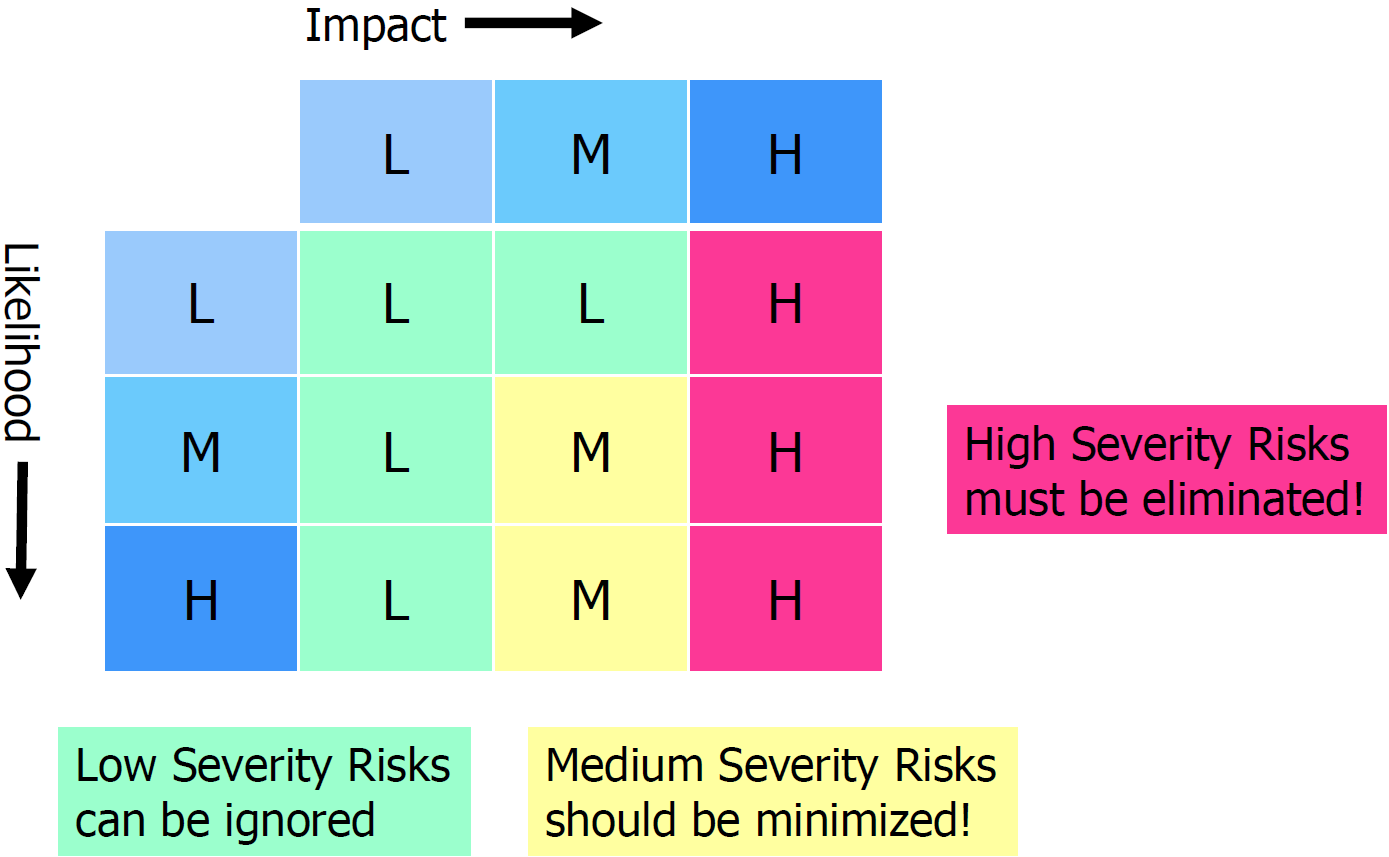
\includegraphics[width=0.6\textwidth]{./img/risk-evaluation}
	\caption{Risiko Evaluations-Matrix}
\end{figure}

\subsubsection{Best Practices}

Es folgen einige Best Practices in der Reihenfolge ihrer Effektivität. Sie können den Kategorien \textbf{K}onstruktiv (white hat) und \textbf{D}estruktiv (black hat) zugeordnet werden.
\begin{easylist}
	& Code Review \textbf{K}
	& Architectural risk analysis (historical knowledge) \textbf{K D}
	& Penetration testing \textbf{D}
	& Risk-based security tests \textbf{D K}
	& Abuse cases \textbf{D K}
	& Security requirements \textbf{K}
	& Security operation \textbf{K}
\end{easylist}

\subsubsection{Fachwissen}
Zum Fachwissen gibt es mehrere Perspektiven. Das Wissen über die Prinzipien, Rahmenbedingungen und Regeln gehören zum Vorgeschriebenen Fachwissen. Dazu gesellt sich die Diagnostischen Fähigkeiten mit dem Wissen über Angriffe, Schwachstellen und Angriffsmuster. Zuletzt benötigt man auch ein Wissen über die Vergangenheit.

\begin{figure}[H]
	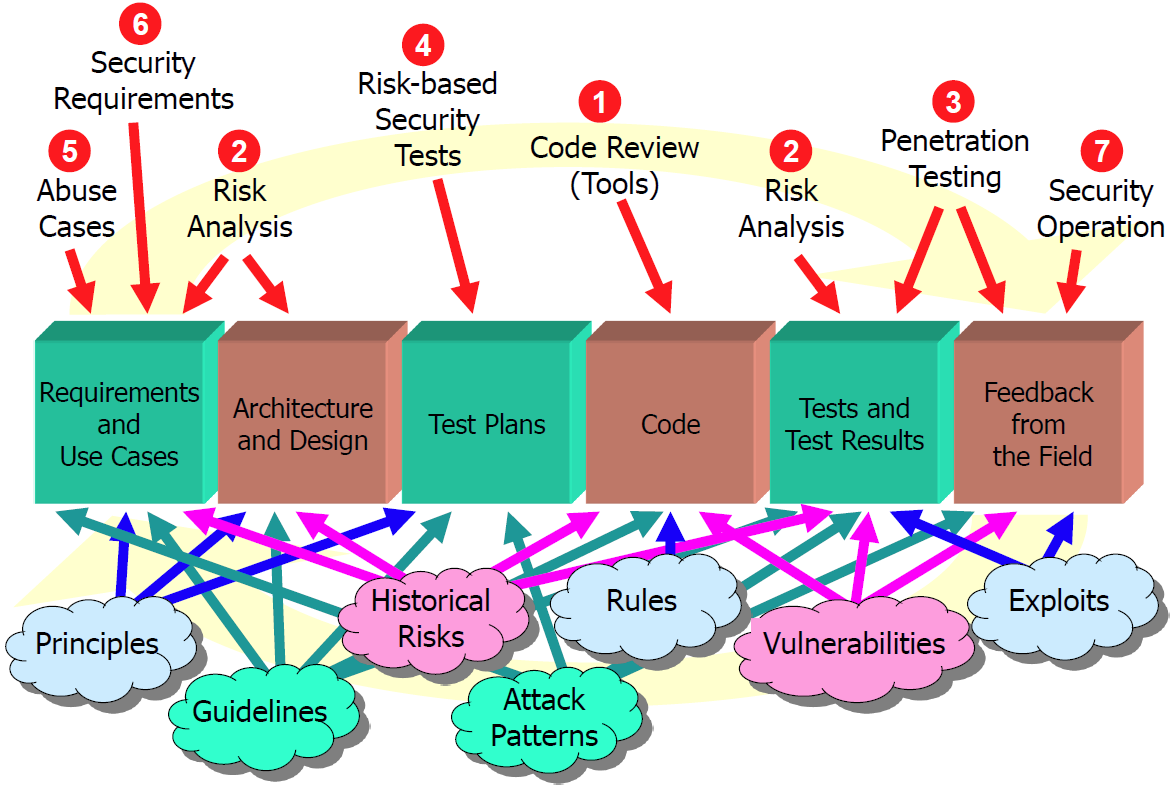
\includegraphics[width=\textwidth]{./img/sdl-best-practice}
	\caption{Best Practices und Fachwissen angewendet auf die Software Artefakte}
\end{figure}

\subsection{Code Analyse}

Für die Analyse von Sourcecode bieten sich mehrere Lösungen an, welche den Quellcode und auch das laufende Programm analysieren und auswerten können. Die ersten Generationen von solchen Analyseprogrammen wurden auch als \textit{Intelligentes Grep} bezeichnet und lieferten viele false positives. In späteren, oft kommerziellen Tools, wurden diese, durch Parsen des Source-Codes, versucht zu minimieren.

Das Wissen aus der Vergangenheit ist in die Regelsätze dieser Software eingeflossen. Jedoch können Probleme in der Softwarearchitektur nicht oder nur selten erkannt werden. Ein manuelles Review ist somit weiterhin nötig. Auch können Abhängigkeiten und falsche Benutzung externer Komponenten nicht korrekt überprüft und erkannt werden.

\subsection{Security Development Lifecycle - SDL}

Der Security Development Lifecycle ist ein Prozess, welcher die \textbf{Sicherheit innerhalb der Softwareentwicklung garantieren} soll. Er wurde von Microsoft entwickelt und gilt als Grundlage, lässt sich also für jede Unternehmensgrösse anpassen. Der SDL umfasst die drei Kernkonzepte \textbf{Schulung}, \textbf{fortwährende Verbesserung der Prozesse} und \textbf{Zurechenbarkeit}.\\
Der SDL sollte auf Projekte mit folgenden Merkmalen angewendet werden:
\begin{easylist}[itemize]
	& Eingesetzt in einem Unternehmen
	& Verarbeitung von personenbezogenen Daten
	& Regelmässige Kommunikation über das Internet oder andere Netzwerke
\end{easylist}
\textbf{Im Prinzip kann der SDL also auf alle Projekte angewendet werden.} Es ist einfacher, diejenigen zu identifizieren, die keinen sicherheitstechnischen Massnahmen benötigen und daher auch auf den SDL verzichten können.\\
Es existieren mehrere Rollen, wovon zwei besonders hervorzuheben sind. Diese lassen sich wiederum weiter unterteilen.
\begin{description}
	\item[Reviewer/Advisory Roles] Diese Rolle soll eine Übersicht über die Sicherheit des Projektes bieten und in der Lage sein, Pläne bezüglich Sicherheit und Datenschutz anzunehmen/abzulehnen. Kann von Internen wie auch externen Personen übernommen werden, aber keine Teammitglieder.
	\item[Team Champions] Diese Rolle ist verantwortlich für den Austausch, Akzeptanz und Verfolgung von minimalen Anforderungen an die Sicherheit und Datenschutz. Sie sind das Gegenstück zu den Advisory Roles und besteht aus Teammitglieder.
\end{description}

Finden die Sicherheitsrelevanten Aktivitäten frühzeitig und innerhalb des Entwicklungsprozesses statt, erhält man den grössten Nutzen daraus.
Um den Microsoft SDL-Prozess einzuhalten müssen die 16 zwingenden Aktivitäten eingehalten werden.

\begin{figure}[H]
	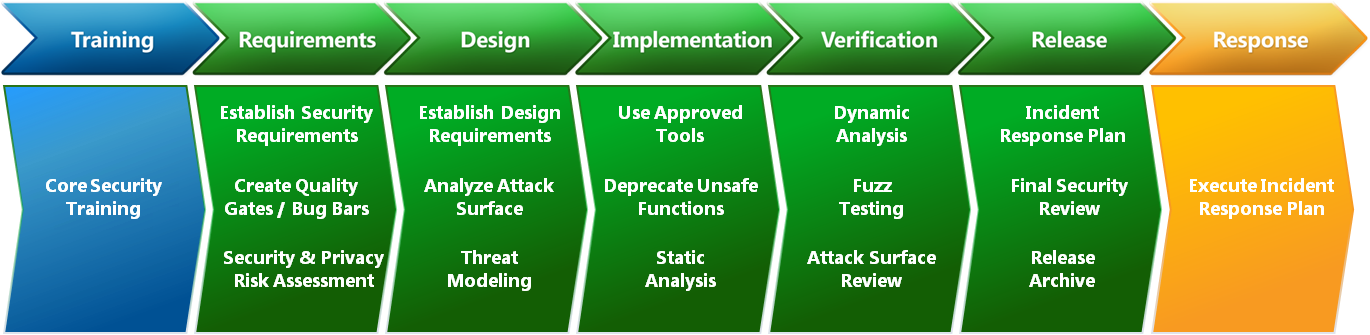
\includegraphics[width=\textwidth]{./img/sdl-overview}
	\caption{Security Development Lifecycle von Microsoft}
\end{figure}

\subsubsection{Training Requirements}
Alle Mitglieder des Entwicklerteams müssen eine Schulung im Bereich Softwaresicherheit erhalten und sich über aktuelle Trends informieren. Die Themen umfassen \textbf{sicheres Design}, \textbf{Modellierung von Bedrohungen}, \textbf{sicheres Coding}, \textbf{Sicherheitstests} und \textbf{Datenschutz}.

\subsubsection{Security Requirements}
Definition von vertrauenswürdigen Anforderungen an das Projekt. Damit können Schlüsselstellen identifiziert werden und die Sicherheit sowie Datenschutz frühzeitig integriert werden. Dies verhindert unnötige Verzögerungen.

\subsubsection{Quality Gates/Bug Bars}
Quality Gates und Bug bars sind minimale Akzeptanzkriterien in Anbetracht der Sicherheit und des Datenschutzes. Das gesamte Team muss sich an die Anforderungen halten, wobei diese nicht dynamisch verändert werden dürfen.
\begin{description}
	\item[Quality Gate] Anforderung an die Code-Qualität bezüglich Compiler-Warnungen, Kommentare, Komplexität, etc.
	\item[Bug Bar] Schwelle für Sicherheitslücken, welche noch im Projekt beim Release enthalten sein dürfen. Z.B. keine Lücken mit der Bewertung "'Kritisch"' oder "'Warnung"'.
\end{description}

\subsubsection{Security and Privacy Risk Assesment}
Beurteilung der Sicherheit- und Datenschutz-Anforderungen von funktionalen Komponenten, welche eine genauere Begutachtung benötigen. Es wird bestimmt, ob weitere Threat Models, Security Design Reviews, Penetration Testing, Zusätzliche Tests und Anforderungen an Fuzz Tests nötig sind.\\
Zusätzlich wird das \textit{Privacy Impact Rating} festgelegt: \textbf{High Privacy Risk} bei der Verarbeitung von personenbezogenen Daten und Einstellungen, \textbf{Medium Privacy Risk} bei Übermittlung anonymisierter Daten und \textbf{Low Privacy Risk}, falls keine Anforderungen für den Datenschutz nötig sind.


\subsubsection{Design Requirements}
Designspezifikationen sollen Sicherheits- und Datenschutz-Funktionen beschreiben, welche direkt dem Benutzer zugänglich sind. Das sind z.B. Funktionen, welche eine Authentisierung oder die Einwilligung des Benutzers erfordern. Gleichzeitig sollten sie auch beschreiben, wie die Sicherheit dieser Funktion implementiert wird.

\subsubsection{Attack Surface Reduction}
Hierbei wird der Zugriff auf das System eingeschränkt und mehrschichtige Abwehrmassnahmen eingeführt. Eng verknüpft mit dem \textit{Threat Modeling}.

\subsubsection{Threat Modeling}
Es werden mögliche Bedrohungen in Betracht gezogen, Diskutiert und Dokumentiert im Kontext der geplanten Umgebung.

\subsubsection{Use Approved Tools}
Im gesamten Team müssen Tools definiert und festgehalten werden, wie damit die Sicherheit überprüft werden. Wie z.B. Compiler- oder Linter-Warnungen.

\subsubsection{Deprecate Unsafe Functions}
Als Team werden die Funktionen und APIs definiert, welche man nicht verwenden darf. Somit können diese dann auch überprüft und durch alternativen ersetzt werden.

\subsubsection{Static Analysis}
Eine skalierbare Möglichkeit zur Analyse des Codes auf Programmierfehler und Einhaltung der Coding-Guidelines. Dies schliesst aber manuelle Reviews nicht aus, diese sollten weiterhin für kritische Bereiche durchgeführt werden.

\subsubsection{Dynamic Program Analysis}
Verifikation während der Laufzeit, dass das Programm auch den Anforderungen entsprechend funktioniert. Es müssen Tools definiert werden, welche ein Fehlverhalten(falsche Berechtigungen) oder die Verwendung von Ressourcen protokollieren.

\subsubsection{Fuzz Testing}
Dynamische Analyse anhand von automatisch generierten Eingaben (absichtlich falsch oder zufällig). Die Strategie fürs Testen wird anhand der Funktionellen- sowie  Design-Spezifikation abgeleitet.

\subsubsection{Threat Model and Attack Surface Review}
Abweichungen der Anwendung von der ursprünglichen Funktionellen- und Design-Spezifikation feststellen und überprüfen, ob Anpassungen nötig sind. Spätestens beim Code-Complete ist eine erneute Analyse notwendig.

\subsubsection{Incident Response Plan}
Damit wird festgehalten, wie bei einem Notfall vorgegangen wird. Zudem sind weitere Informationen enthalten, welche für die Behebung und Verarbeitung hilfreich sind.
\begin{itemize}
	\item Ansprechperson für den ersten Kontakt sowie, wenn vorhanden, auch ein Entwicklerteam.
	\item Ansprechperson mit Entscheidungsgewalt, verfügbar 24/7.
	\item Sicherheitsrelevante Informationen von Code anderer Entwickler-Teams.
	\item Sicherheitsrelevante Informationen von Third-Party-Komponenten, dessen Version, Dateinamen, Kontaktdaten und Vertragsinformationen, falls vorhanden.
\end{itemize}

\subsubsection{Final Security Review}
Die eigentliche Kontrolle vor dem Release, ob die Software allen im Prozess definierten Anforderungen entspricht und die Sicherheitsaktivitäten eingehalten wurden. Hier werden die Gesammelten Informationen aus Threat Models, exception requests, Ausgabe der Tools und Performanz mit den Quality Gates und Bug Bar verglichen. Daraus ergibt sich dann das Resultat \textbf{FSR bestanden}, \textbf{FSR bestanden mit Ausnahmen} oder \textbf{FSR mit Eskalation}.

\subsubsection{Release/Archive}
Die Software ist aus Sicht des SDL komplett und kann nach Bestätigung des Sicherheitsberaters freigegeben werden. Für jede High Privacy Risk wird auch eine Bestätigung des Datenschutzbeauftragten benötigt.
Alle im Prozess erzeugten Artefakte müssen archiviert werden, um eine Wartung nach dem Release zu ermöglichen.

\subsubsection*{Optionale Sicherheitsaktivitäten}
Die zuvor beschriebenen Sicherheitsaktivitäten sind nur das Minimum und können noch weiter ergänzt werden.\\
Ein \textbf{manuelles Code-Review} wird eingesetzt, wenn besonders sensitive Daten verarbeitet oder gespeichert werden. Es macht auch Sinn, Implementationen von kryptographischen Funktionen auf ihre Korrektheit zu überprüfen.\\
In einem \textbf{Penetration Testing} wird als Whitebox-Analyse die Sicherheit durch Spezialisten mit der Vorgehensweise von Hackern durchgeführt. Sie bieten zusätzliche Anhaltspunkte und ergänzen Code-Reviews.\\
Als weiterer Schritt kann auch die \textbf{Analyse auf Schwächen in vergleichbaren Anwendungen} gesehen werden. Da oftmals die Informationen über Schwachstellen im Internet verfügbar sind, können diese mit der eigenen Anwendung verglichen werden, ob diese auch zutreffen.

\section{Application Security Basics}

\subsection{HTTP Basics}

HTTP ist \textbf{Zustandslos}: Der Client sendet eine Anfrage (\textbf{Request}) an den Server, welcher ihn verarbeitet und anschliessend das Resultat als Antwort (\textbf{Response}) zurücksendet.\\

\begin{figure}[H]
	\centering
	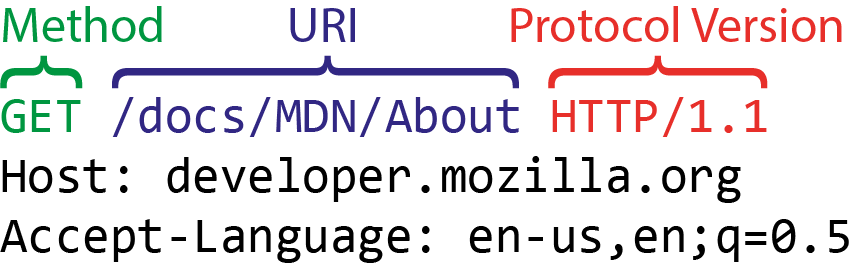
\includegraphics[width=0.38\textwidth]{./img/http-head}
	\caption{HTTP Header}
\end{figure}

Zwischen HTTP GET und POST gibt es einen wesentlichen Unterschied. Da der Server die URI in der Regel mitloggt, werden auch die \textbf{Parameter des GET-Request mitgeloggt}. Beim POST-Request geschieht dies nicht, da sich die Parameter anstatt in der URI im Body befinden. Dies ist auch bei Proxies zu beachten. Eine \textbf{Response} ist beinahe Identisch zum Request. Die erste Zeile enthält nun das Protokoll, Statuscode und Statusbeschreibung (HTTP/1.1 200 OK).

\begin{figure}[H]
	\centering
	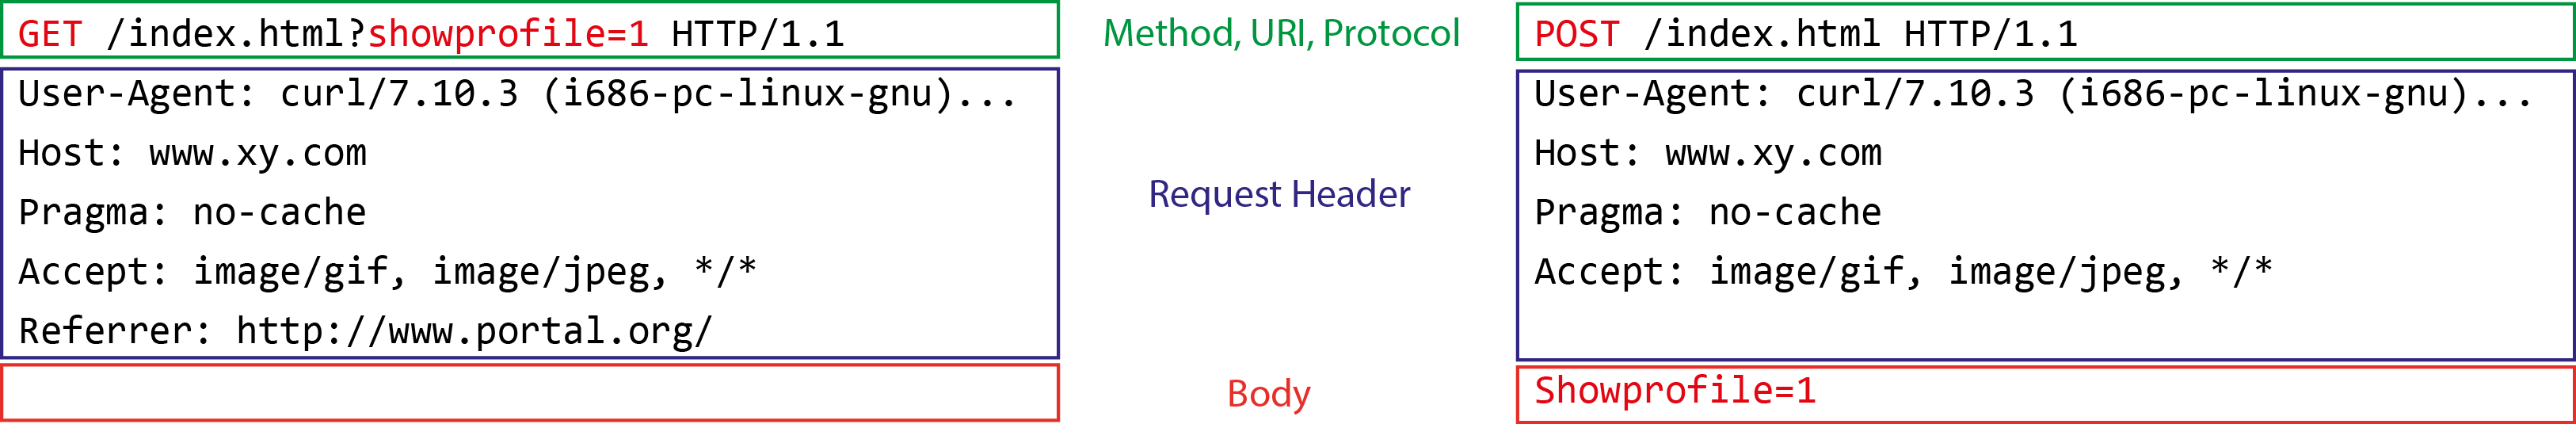
\includegraphics[width=\textwidth]{./img/http-full-request}
	\caption{Beispielrequests für GET und POST}
\end{figure}

\begin{table}[H]
	\begin{tabularx}{\textwidth}{l|X}
		\textbf{HTTP Methode} & \textbf{Verwendung}\\ \hline
		GET		& normale verwendung *\\ \hline
		POST	& übermittlung von Daten (Login, Formulare) *\\ \hline
		HEAD	& Suchmaschinen (Head of page) *\\ \hline
		PUT		& Upload von Dateien (webdav, RESTful)\\ \hline
		DELETE	& Löschen von Dateien (webdav, RESTful)\\ \hline
		OPTIONS	& Auflistung verfügbarer Methoden auf Server\\ \hline
		TRACE	& Debugging in Webserver\\ \hline
	\end{tabularx}
	\caption{Übliche HTTP Methoden (* meist verwendet)}
\end{table}


\begin{table}[H]
	\begin{tabularx}{\textwidth}{l|p{100pt}|X}
		\textbf{Statuscode} & \textbf{Nachricht} & \textbf{Bedeutung}\\ \hline
		\multicolumn{3}{c}{2xx - Erfolgreich} \\ \hline
		200 & OK & Anfrage erfolgreich bearbeitet, Ergebnis in der Antwort enthalten. \\ \hline
		\multicolumn{3}{c}{3xx - Umleitung} \\ \hline
		301 & Moved Permanently & Header "'Location: http://other-site/"' \\ \hline
		302 & Moved Temporarily & Header "'Location: http://other-site/"'; Alternativ 303 oder 307 möglich \\ \hline
		\multicolumn{3}{c}{4xx - Clientfehler} \\ \hline
		400 & Bad Request & Anfrage war fehlerhaft aufgebaut \\ \hline
		401 & Unauthorized & Authentifizierung nötig \\ \hline
		403 & Forbidden & Mangelnde Berechtigung des Clients \\ \hline
		404 & Not Found & Angeforderte Ressource nicht gefunden \\ \hline
		405 & Method Not Allowed & \\ \hline
		408 & Request Timeout & \\ \hline
		\multicolumn{3}{c}{5xx - Serverfehler} \\ \hline
		500 & Internal Server Error & Allgemeiner Serverfehler \\ \hline
		501 & Not Implemented & Funktionalität wird vom Server nicht bereitgestellt \\ \hline
		502 & Bad Gateway & Proxy hat ungültige Antwort erhalten \\ \hline
		503 & Service Unavailable & Service steht temporär nicht zur verfügung \\ \hline
	\end{tabularx}
	\caption{Übliche HTTP Statuscodes, \url{https://de.wikipedia.org/wiki/HTTP-Statuscode}}
\end{table}

\subsection{Redirect after succesful login}
Unter diesem Namen verbirgt sich ein Pattern, um die "'\textbf{Back Button Relogin Vulnerability}"' zu adressieren. Ohne Anwendung dieses Patterns besteht die Möglichkeit, dass nach mehrmaligem Klick auf Zurück die eingegebenen Logindaten erneut an den Server übertragen werden. Bei Fehlschlag des Logins kann mittels eines gewöhnlichen \textit{200 OK} um eine erneute Eingabe gebeten werden.

\begin{figure}[H]
	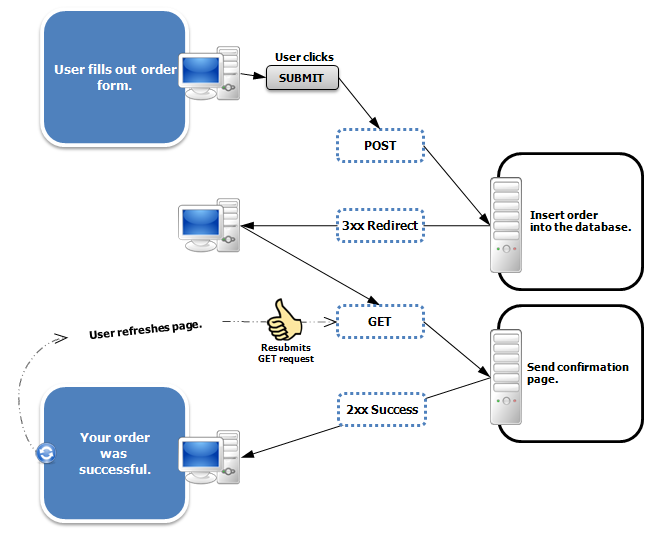
\includegraphics[width=\textwidth]{./img/PostRedirectGet_DoubleSubmitSolution}
	\caption{Redirect after succesful login}
\end{figure}

Es gibt dabei mehrere Varianten für den Redirect:
\begin{easylist}
	& Type 1 (302 Moved Temporarily)
	&& HTTP Response Status 302
	&& HTTP Response Header "'Location: http://other-site/"'
	& Type 2 (200 OK)
	&& HTTP Response Status 200
	&& HTTP Response Header "'Refresh: 0; URL=http://other-site/"'
	& Type 3 (200 OK)
	&& HTTP Response Page
	&& Meta-Tag "'Refresh"'
	& Type 4 (Javascript)
	&& Client-Seitiger Code (z.B. "'document.location=\ldots"')
\end{easylist}

\subsection{HTTP Session Management}
Serverseitig wird eine Speicherstruktur erstellt, um Session-Daten zu speichern. Der Client erhält ein Schlüssel zu dieser Struktur, auch bekannt als \textit{SessionId}.\\
Bei jeder Anfrage des Clients an den Server muss dieser die \textit{SessionId} mitgeben, damit der Server auf die Daten der Session zugreifen kann. Dazu gibt es mehrere Varianten, wo sich die SessionId befindet (\textbf{Session Locations}):
\begin{easylist}[itemize]
	& URI
	&& Sichtbar in Logs
	&& Problematisch beim Caching
	& Request Header
	&& Cookie, NTLM, BasicAuth
	& Body
	&& Als Hidden Field
	&& Kaum verbreitet
\end{easylist}

\subsection{Cookies}

\begin{verbatim}
Set-Cookie: PREF=ID=2744d38c32b2ec68:LD=de:TM=1094031009
expires=Sun, 17-Jan-2038 19:14:07 GMT; path=/; domain=.google.ch
\end{verbatim}

\begin{figure}[H]
	\centering
	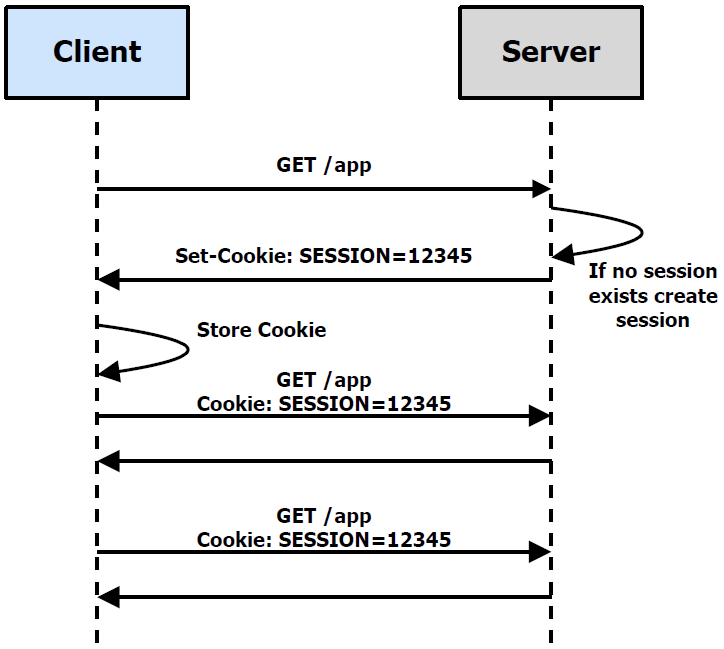
\includegraphics[width=0.6\textwidth]{./img/cookie-creation}
	\caption{Cookie erzeugung über HTTP Request Header}
\end{figure}

\subsubsection{Cookie Attribute}

\begin{easylist}[itemize]
	& \textbf{Name=Content} (Key, value pair)
	&& Name: Cookie Name
	&& Content: Cookie Value
	&& Beispiel: jsessionid=klrezbxur234kls
	& \textbf{Domain}
	&& Ort wohin das Cookie gesendet werden kann.
	&& Default: Cookie wird nur an den Server gesendet, von dem es stammt.
	& \textbf{Path}
	&& URL-Path wohin das Cookie gesendet werden kann.
	&& Default: Cookie wird nur an den Pfad gesendet, von dem es stammt.
	& \textbf{Secure}
	&& Cookie wird nur über HTTPS übermittelt.
	&& Default: insecure
	& \textbf{Expire}
	&& Gültigkeit des Cookies.
	&& Default: wird nicht persistiert, nur Browsersession.
	& \textbf{HttpOnly}
	&& Cookie kann nicht von JavaScript verwendet werden.
	&& Default: nicht vorhanden, JavaScript kann mit document.cookie darauf zugreifen.
\end{easylist}

Wann ein Cookie \textbf{an den Server gesendet} wird, ist abhängig von mehreren Attributen: Domain, Path, Secure und Expire.\\
Das HttpOnly Attribut bietet ein Schutz gegenüber XSS, wobei es dem JavaScript, welches eingeschleust wurde, verhindert wird, auf das Cookie zuzugreifen.

\subsubsection{SSL Session ID}
Mithilfe der \textit{SSL Session ID} können SSL-Session weiter verwendet werden, ohne einen erneuten Handshake durchzuführen. Ähnlich wie bei Cookies werden diese zu beginn der Anfrage an den Server übermittelt, welcher den zur ID passenden symmetrischen Schlüssel besitzt.\\
Der gesamte Payload des SSL-Pakets ist verschlüsselt, man sieht also weder die URL noch andere Inhalte des HTTP-Paket.

\subsection{Cross Site Scripting - XSS}
Die Gefahr für XSS entsteht, wenn Benutzereingaben unzureichend gefiltert werden und unverändert wieder an andere Benutzer ausgeliefert werden. Dies ermöglicht z.B. die Übernahme von Sessions, HTML- oder JS-Injection, Exploit injection oder Keylogging.\\
Es werden drei Typen von Attacken unterschieden:
\begin{description}
	\item[Stored] Das injizierte Skript ist permanent auf dem Zielserver gespeichert, z.B. in Form von Forumsbeiträgen.
	\item[Reflected] Das Skript wird nicht auf dem Zielserver gespeichert, der Angreifer muss aber eine URL präparieren und diese dem Opfer unterjubeln. Dies ist z.B. über eine Suchanfrage möglich.
	\item[DOM based] Angreifer muss eine URL präparieren, welche dann im Client direkt ausgelöst wird. Server wird dabei nicht aufgerufen, clientseitige Validierung nötig.
\end{description}

Mögliche \textbf{Gegenmassnahmen} sind:
\begin{description}
	\item[HTML entities] Encoding vor dem Speichern und bei der Ausgabe.
	\item[HTTP Only Cookies] Auslesen über JS nicht möglich.
	\item[CSP] Content Security Policy: \lstinline|script-src 'self'|
\end{description}

\subsection{Same Origin Policy}
Die damit wird verhindert, dass Javascript (auch Flash, Java Applet, etc.) auf DOM und Cookies zugreifen kann. Nur bei der Übereinstimmung von \textbf{Protokoll, Host und Port} wird dies erlaubt.\\
Wird nun aber in der Ursprungs-Seite das 3rd-Party-Script durch \lstinline|<script src="...">| geladen, so kann es auf das Cookie der Ursprungs-Seite zugreifen.\\
Die Übermittlung von Daten an fremde Seiten kann dann über Bild-Tags erfolgen, da diese nicht der SOP unterliegen.\\
Wird der Javascript-Code über die URL injiziert, so spricht man von \textbf{Reflected XSS}. Der XSS-Schutz im Browser kann dies verhindern, aber nicht bei \textbf{Stored XSS}.

\subsection{Cross Origin Resource Sharing - CORS}
Damit schützt sich nicht der eigentliche Webseitenbetreiber, sondern ein Serivce-Provider, welcher Daten für den Betreiber bereitstellt. Anfragen an den Service-Provider enthalten ein Header \lstinline|Origin: http://foo.example.com|. Die Antwort darauf den Header \lstinline|Access-Control-Allow-Origin: http://foo.example.com| (Wildcards sind auch möglich).

\subsubsection{CORS Preflighted Request}

Der Preflight wird ausgeführt, falls eine der folgenden Bedingungen zutrifft:
\begin{easylist}[itemize]
	& Verwendung einer Methode ausser GET, HEAD oder POST.
	& POST fordert Daten mit einem anderen Content-Type als \lstinline|application/x-www-form-urlencoded, multipart/form-data oder text/xml| an
	& POST sendet Daten mit einem XML-Payload zum Server.
\end{easylist}

\begin{figure}[H]
	\centering
	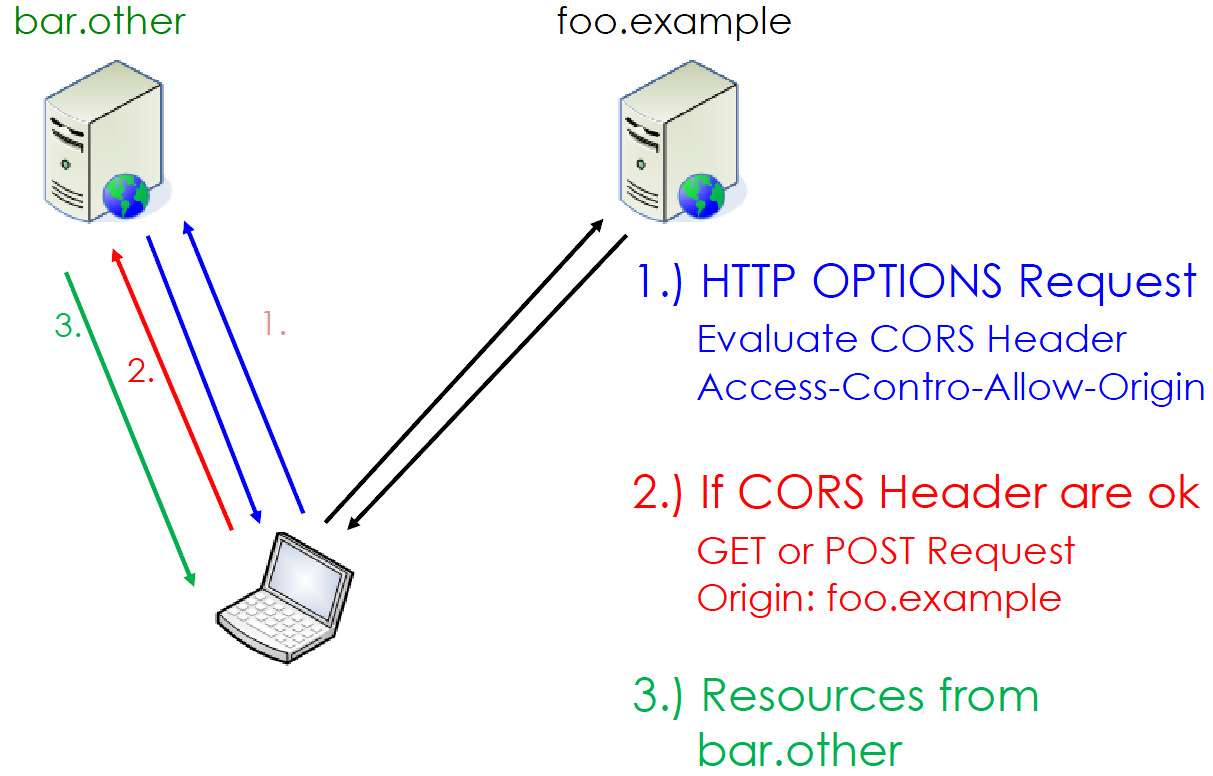
\includegraphics[width=0.6\textwidth]{./img/cors-preflight}
	\caption{Vorgehen beim CORS Preflight}
\end{figure}

Standardmässig werden bei XMLHttpRequests aufrufen keine Credentials/Cookies mitgeschickt. Um dies zu forcieren, muss ein spezielles Flag (withCredentials) auf dem Request-Objekt gesetzt werden.

\subsection{Content Security Policy - CSP}
Dahinter versteckt sich ein Sicherheitskonzept, um XSS und diverse andere Angriffe wie Clickjacking und Code Injection, durch einschleusen von Daten in Webseiten zu verhindern. Es wird als HTTP-Header-Field \textit{Content-Security-Policy} und bei IE 10+ \textit{X-Content-Security-Policy} unterstützt.
Dadurch kann der Server bestimmen von welchem Origin Content geladen werden darf. Trifft auf ein Element mehrere CSPs zu, wird immer die restriktivste benutzt!

\begin{lstlisting}[caption=Starter Policy für CSP-Header, language={}]
Content-Security-Policy: default-src 'none'; script-src 'self'; connect-src 'self'; img-src 'self'; style-src 'self';
\end{lstlisting}

Das Vorgehen beim erstellen einer neuen CSP ist wie folgt:
\begin{enumerate}
	\item CSP-Header bei allen Requests hinzufügen mit Policy \lstinline[language=clean]|default-src 'none'|
	\item Verstösse in der Browser-Konsole anschauen
	\item Nötige Quellen zur Policy hinzufügen
\end{enumerate}

CSP hat folgende Defaults aktiviert:
\begin{enumerate}
	\item Keine Inline Javascript-Snippets. Nur aus Files 
	\item Keine JS-URLs wie javascript:http://url
	\item Eventhandling-Attribute sind deaktiviert (zum Beispiel document.click())
	\item Funktion eval() ist deaktiviert
	\item Der Konstruktor von function() ist deaktiviert
	\item URIs sind nur für Bilder erlaubt
\end{enumerate}

\subsection{X-Frame-Headers}
Als HTTP-Header-Feld eingesetzt dient es als Schutz vor \textbf{Clickjacking}-Attacken. Dabei wird dem Opfer ein Frame über ein anderen Inhalt gelegt und so versucht, durch Klicken Aktionen auf dem dahinterliegenden Objekt auszuführen.\\
\textbf{CSP hat Vorrang} vor X-Frame-Headers, weil die Unterbindung von Frames seit Version 2.0 dort auch integriert ist.

\begin{lstlisting}[caption=Clickjacking mittels X-Frame-Options unterbinden, language={}]
X-Frame-Options: DENY
\end{lstlisting}

\subsection{HTTP Strict Transport Security - HSTS}
Ein Sicherheitsmechanismus für HTTPS-Verbindungen. Er soll vor Aushebelung der Verbindungsverschlüsselung durch eine Downgrade-Attacke als auch vor Session Hijacking schützen. Durch die Angabe des Header-Feldes wird jede weitere Verbindung bis zum erreichen des \textit{max-age} als \textbf{HTTPS erzwungen}, auch wenn die Links z.B. auf HTTP lauten. Zusätzlich wird eine Verbindung mit dem Server verhindert, sobald \textbf{Zertifikatsprobleme} auftauchen.\\

Google Chrome wie auch andere Browser verwenden \textbf{HSTS-Preload-Listen}. Damit wird die Limitierung des \textit{trust on first use}-Prinzip für eine definierte Liste von Domains umgangen.

\begin{lstlisting}[language={},caption=HSTS-Header]
Strict-Transport-Security: max-age=31536000
\end{lstlisting}

\subsection{X-XSS-Protection}
Dieser Header aktiviert den XSS-Schutz im Browser, jedoch kann dieser nur Reflected XSS erkennen. Bisher wird es nur von IE, Chrome und Safari unterstützt. In diesen Browser sollte er jedoch standardmässig bereits aktiviert sein.

\begin{lstlisting}[language={},caption=Beispiel des X-XSS-Protection Headers]
X-XSS-Protection: 1; mode=block
\end{lstlisting}

\subsection{HTTP Public Key Pinning - HPKP}
Eine Erweiterung für HTTP, das dem Webclient mitteilt, einen spezifischen kryptographischen Schlüssel mit einem bestimmten Webserver in Verbindung zu bringen. So sollen Man-in-the-Middle-Angriffe mit gefälschten Zertifikaten vermieden werden.\\

Google Chrome wie auch Firefox verwenden \textbf{Preload-Listen}. Damit wird die Limitierung des \textit{trust on first use}-Prinzip für eine definierte Liste von Domains umgangen.

\begin{lstlisting}[language={},caption=Beispiel des HPKP-Headers]
Public-Key-Pins: pin-sha256="base64=="; max-age=expireTime [; includeSubdomains][; report-uri="reportURI"]
\end{lstlisting}

\section{OWASP Top 10}
Die OWASP Top 10 sind die zehn wohl wichtigsten Schwachstellen von Anwendungen, welche aus dem \textit{Open Web Application Security Project} hervor ging.\\

Die aktuellste Version ist 2013 in \fnurl{http://owasptop10.googlecode.com/files/OWASP\%20Top\%2010\%20-\%202013.pdf}{Englisch} erschienen und in mehrere Sprachen übersetzt, unter anderem auch \fnurl{https://www.owasp.org/images/4/42/OWASP_Top_10_2013_DE_Version_1_0.pdf}{Deutsch}. Die hier aufgeführten Kurzbeschreibungen stammen ebenfalls aus der deutschen Version.

\subsection{Injection}
Injection-Schwachstellen (SQL-, OS- oder LDAP-Injection) treten auf wenn nicht vertrauenswürdige Daten als Teil eines Kommandos oder einer Abfrage von einem Interpreter verarbeitet werden. Ein Angreifer kann Eingabedaten dann so manipulieren, dass er nicht vorgesehene Kommandos ausführen oder unautorisiert auf Daten zugreifen kann.

\subsection{Broken Authentication and Session management}
Anwendungsfunktionen, die die Authentifizierung und das Session-Management umsetzen, werden oft nicht korrekt implementiert. Dies erlaubt es Angreifern Passwörter oder Session-Token zu kompromittieren oder die Schwachstellen so auszunutzen, dass sie die Identität anderer Benutzer annehmen können.

\subsection{Cross-Site-Scripting - XSS}
XSS-Schwachstellen treten auf, wenn eine Anwendung nicht vertrauenswürdige Daten entgegennimmt und ohne entsprechende Validierung oder Umkodierung an einen Webbrowser sendet. XSS erlaubt es einem Angreifer Scriptcode im Browser eines Opfers auszuführen und somit Benutzersitzungen zu übernehmen, Seiteninhalte zu verändern oder den Benutzer auf bösartige Seiten umzuleiten.

\subsection{Insecure Direct Object References}
Unsichere direkte Objektreferenzen treten auf, wenn Entwickler Referenzen zu internen Implementierungsobjekten, wie Dateien, Ordner oder Datenbankschlüssel von aussen zugänglich machen. Ohne Zugriffskontrolle oder anderen Schutz können Angreifer diese Referenzen manipulieren um unautorisiert Zugriff auf Daten zu erlangen.

\subsection{Security Misconfiguration}
Sicherheit erfordert die Festlegung und Umsetzung einer sicheren Konfiguration für Anwendungen, Frameworks, Applikations-, Web- und Datenbankserver sowie deren Plattformen. Sicherheitseinstellungen müssen definiert, umgesetzt und gewartet werden, die Voreinstellungen sind oft unsicher. Des Weiteren umfasst dies auch die regelmässige Aktualisierung aller Software.

\subsection{Sensitive Data Exposure}
Viele Anwendungen schützen sensible Daten, wie Kreditkartendaten oder Zugangsinformationen nicht ausreichend. Angreifer können solche nicht angemessen geschützten Daten auslesen oder modifizieren und mit ihnen weitere Straftaten, wie beispielsweise Kreditkartenbetrug, oder Identitätsdiebstahl begehen. Vertrauliche Daten benötigen zusätzlichen Schutz, wie z.B. Verschlüsselung während der Speicherung oder Übertragung sowie besondere Vorkehrungen beim Datenaustausch mit dem Browser.

\subsection{Missing Function Level Access Control}
Die meisten betroffenen Anwendungen realisieren Zugriffsberechtigungen nur durch das Anzeigen oder Ausblenden von Funktionen in der Benutzeroberfläche. Allerdings muss auch beim direkten Zugriff auf eine geschützte Funktion eine Prüfung der Zugriffsberechtigung auf dem Server stattfinden, ansonsten können Angreifer durch gezieltes Manipulieren von Anfragen ohne Autorisierung trotzdem auf diese zugreifen.

\subsection{Cross-Site Request Forgery - CSRF}
Ein CSRF-Angriff bringt den Browser eines angemeldeten Benutzers dazu, einen manipulierten HTTP-Request an die verwundbare Anwendung zu senden. Session Cookies und andere Authentifizierungsinformationen werden dabei automatisch vom Browser mitgesendet. Dies erlaubt es dem Angreifer Aktionen innerhalb der betroffen Anwendungen im Namen und Kontext des angegriffen Benutzers auszuführen.

\subsection{Using Components with Known Vulnerabilities}
Komponenten wie z.B. Bibliotheken, Frameworks oder andere Softwaremodule werden meistens mit vollen Berechtigungen ausgeführt. Wenn eine verwundbare Komponente ausgenutzt wird, kann ein solcher Angriff zu schwerwiegendem Datenverlust oder bis zu einer Serverübernahme führen. Applikationen, die Komponenten mit bekannten Schwachstellen einsetzen, können Schutzmassnahmen unterlaufen und so zahlreiche Angriffe und Auswirkungen ermöglichen.

\subsection{Unvalidated Redirects and Forwards}
Viele Anwendungen leiten Benutzer auf andere Seiten oder Anwendungen um oder weiter. Dabei werden für die Bestimmung des Ziels oft nicht vertrauenswürdige Daten verwendet. Ohne eine entsprechende Prüfung können Angreifer ihre Opfer auf Phishing-Seiten oder Seiten mit Schadcode um- oder weiterleiten.

\section{Identity and Access Management}

Unter \textbf{Federated Identity Management} gehören Abkommen, Standards und Technologien für Identitäten und Berechtigungen portabel über autonome Identitätsdomänen. Die \textit{Föderation} (Zusammenschluss) ermöglicht es, die Identitätsinformationen von verschiedenen Systemen transparent und sicher auszutauschen, um damit auf Sicherheitsebene zusammenarbeiten zu können.

\subsection[AAI]{Authentication \& Authorization Infrastructure - AAI}
\textbf{Ohne eine einheitliche AAI} benötigt jede zu schützende Ressource eine separate Benutzer-Administration und -Authentifikation. Probleme/Nachteile ohne AAI:
\begin{easylist}
	& Aufwändige und fehleranfällige Registration auf für jede einzelne Ressource
	& Unzuverlässige und veraltete Daten
	& Verschiedene Logins/Passwörter
	& Gewisse Ressourcen werden gar nicht erst benötigt
	& Ressorucen sind meist nur durch IP-Adressen geschützt
\end{easylist}

\textbf{Mit einer AAI} muss sich der Benutzer nur noch an einer Stelle Authentifizieren. Die Authentifizierung wird dann an den verschiedenen Ressourcen für die Autorisierung benötigt. Vorteile durch AAI:
\begin{easylist}
	& Keine Registration pro Ressource nötig
	& Einheitliche Login-Prozedur
	& Neue Ressourcen können leicht hinzugefügt werden
	& Standortunabhängig
	& Weniger Kennwörter zu merken
\end{easylist}


\begin{figure}[H]
	\centering
	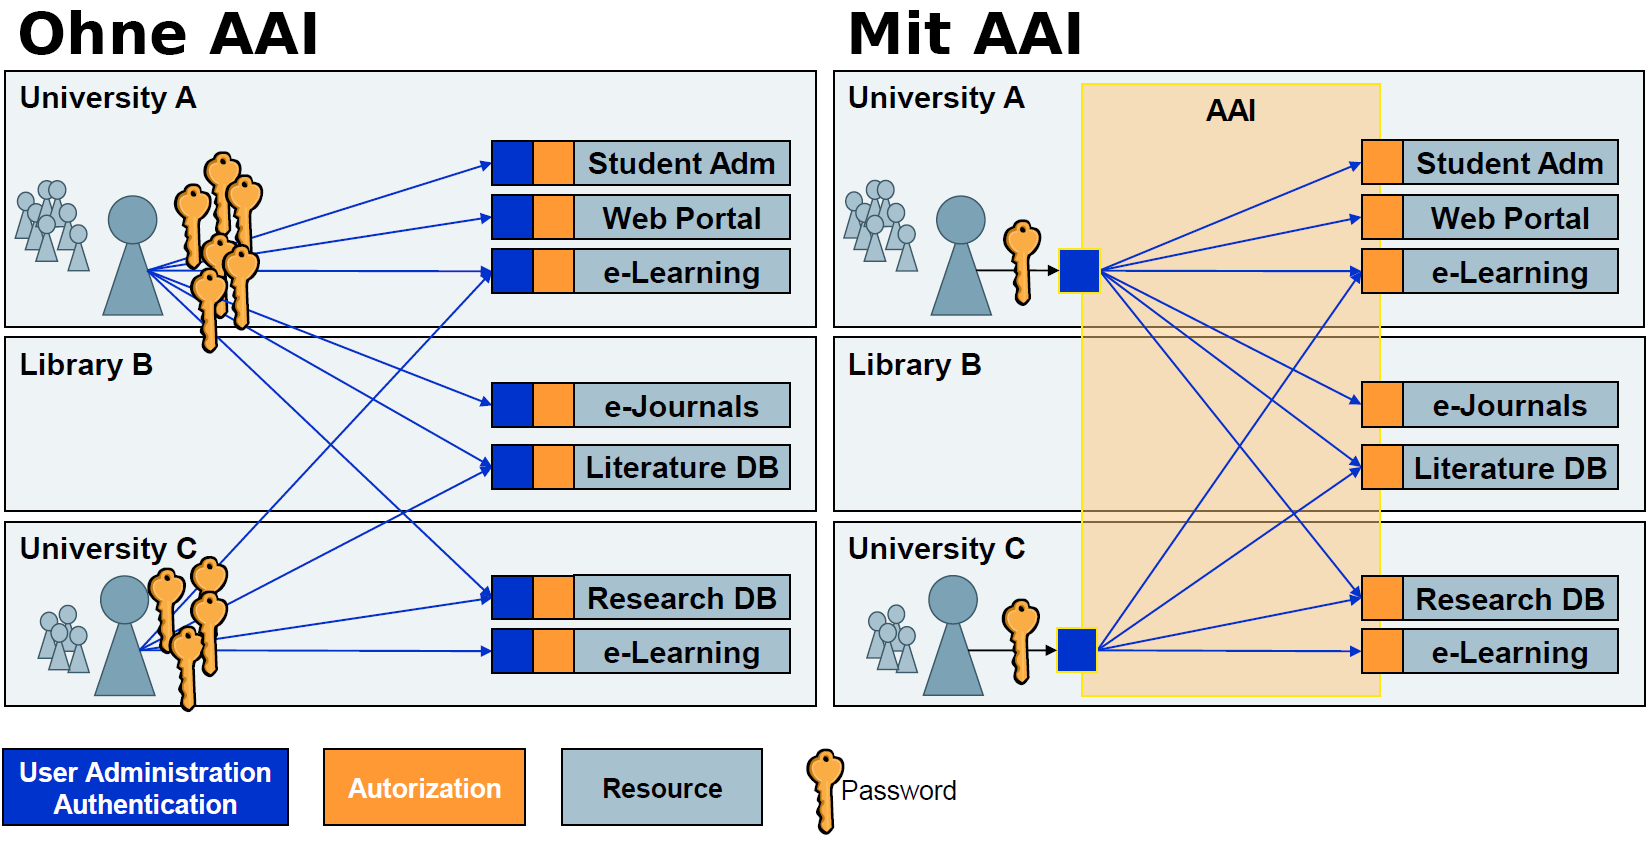
\includegraphics[width=\textwidth]{./img/AAI-example}
	\caption{Exemplarische Übersicht von AAI (Source: switch.ch/aai)}
\end{figure}

\subsubsection{Shibboleth}
Eines der weit verbreiteten AAI, welches die Authentifizierung von Classic Web-Services über die Protokolle \textbf{SOAP, XML und SAML} übernimmt unter Verwendung von \textbf{http}.\\
Basiert auf \textbf{SAML-Assertions} (Security Assertion Markup Language) ausgestellt von vertrauten Home-Organisationen (\textbf{Identity Providers}), welche von Ressourcen (\textbf{Service Providers}) aus dem Verbund akzeptiert werden.

\begin{figure}[H]
	\centering
	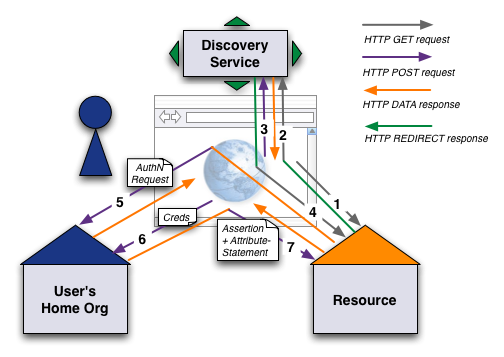
\includegraphics[width=0.7\textwidth]{./img/shibboleth-login}
	\caption{Vollständige Loginprozedur mit Shibboleth (Source: switch.ch/aai)}
\end{figure}

Ein \textbf{Beispiel für AAI} mittels Shibboleth ist das System von SWITCH für Universitäten, mit dem man sich z.B. bei Unterrichtsplattformen oder Online-Shops mit dem Login der Uni-/Fachhochschule anmelden kann.\\
Dieses System übermittelt zudem \textbf{zusätzliche Attribute} zum authentifizierten Benutzer, wie etwa seine Mail-Adresse oder SwissEduPersonUniqueID.\\

Der Standard \textbf{XML Signature Syntax and Processing} erlaubt die Signierung, Integritätsprüfung und Nachrichtenauthentifizierung.\\
Der Standard \textbf{XML Encryption Syntax and Processing} erlaubt die Verschlüsselung von Daten (sogar teile des XML-Dokumentes) innerhalb eines XML-Dokumentes.\\
Der Standard \textbf{Secure Assertion Markup Language 2.0} kombiniert den XML Signature Syntax und XML Encryption Syntax in einem Dokument mit Authentifikation Attriuten und Autorisation. Das resultierende XML-Dokument ist eine portable Identität für Single Sign-On Web Services.\\
Die Verwendung von SAML bringt als Vorteil mit sich, dass \textbf{bestehende Enterprise-Anwendungen} direkt integriert werden können. Das zu grunde liegende XML bringt aber dennoch etwa \textbf{90\% Overhead} mit sichs.\\

Über die Architektur von \textbf{SuisseID} lässt sich so z.B. auch die \textbf{Alters-Verifikation} sicherstellen, da für die Ausstellung eine Identitätsprüfung durchgeführt wird.

\subsubsection{OAuth2}
Wurde entworfen für neuere Protokolle wie \textbf{REST und JSON}, kommuniziert über \textbf{https}. Es gibt keine eingebauten Sicherheits-Funktionen, diese wird komplett durch TLS (z.B. https) übernommen. Die Funktionsweise ist \textbf{vergleichbar mit Kerberos}.\\

\begin{description}
	\item[Resource Owner] Benutzer
	\item[Resource Server] Die API
	\item[Authorization Server] Autorisiert den Benutzer, oftmals auf dem selben Server wie Resource Server.
	\item[Client] Thirt-Party application, welche auf die API zugreifen möchte.
\end{description}


\begin{figure}[H]
	\centering
	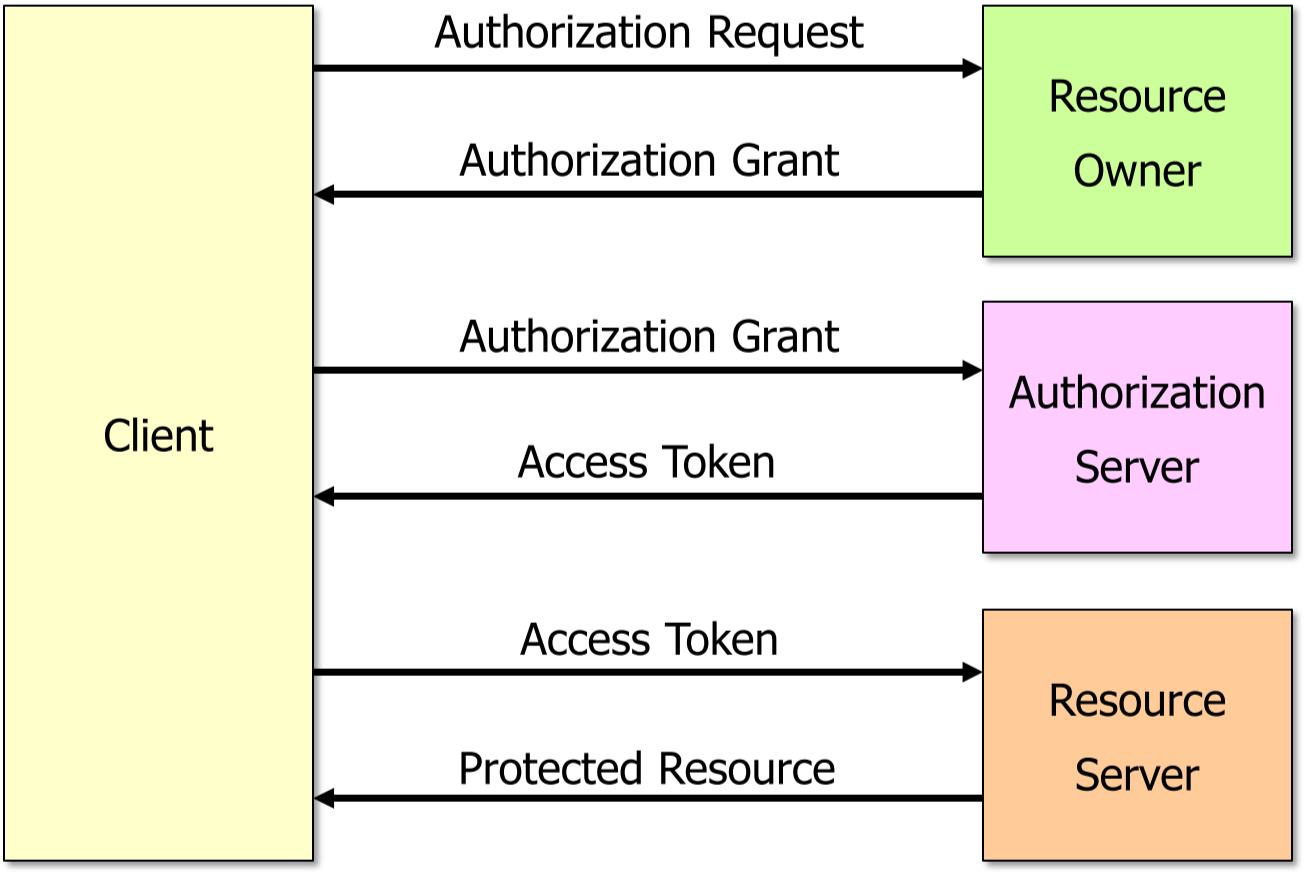
\includegraphics[width=0.5\textwidth]{./img/oauth2-example}
	\caption{Beispiel eines Zugriffs auf geschützte Ressourcen mittels OAuth2}
\end{figure}

Man kann OAuth2 nicht als zuverlässige Benutzerauthentisierung zählen. OpenID connect versucht aber diese Probleme zu lösen.\\

Jeder Anbieter setzt eine andere Versionen davon ein oder sogar eine eigene Implementierung.

\subsubsection{OpenID Connect}
\begin{easylist}[itemize]
	& OpenID Connect 1.0 is a simple identity layer on top of OAuth 2.0.
	& OpenID Connect 1.0 specifies a REST-based http API, using JSON as a data format..
	& OpenID Connect 1.0 uses a JSON Web Token (JWT) which can be signed using JSON Web Signature (JWS) and optionally encrypted using JSON Web Encryption (JWE).
	& OpenID Connect 1.0 is used by Google+ Sign-In.
\end{easylist}

\section{Web Entry Server}
Ohne Massnahmen werden mehrere Verbindungen direkt zu den Applikationsserver in der DMZ gemacht. Um dies zu verhindern wird eine \textbf{Web Entry Server} eingesetzt, welcher ein modifizierter Apache Web Server ist.

Insgesamt kann dieser Server dann auch als \textbf{Web Application Firewall} (WAF) bezeichnet werden, und folgende Funktionen übernehmen:

\begin{easylist}[itemize]
	& Network Filter Level
	& SSL Termination
	& Protocol Validation and Rebuilding
	& Character Encoding and Unicode Verficatoin
	& White/Black List Filter
	& Cookie Protection
	& URL Encrypting
	& Smart Form Protection
	& Response Content Filter
	& Response Rewriting
	& Pre-Authentication
\end{easylist}

\subsection{Reverse Proxy}
Ein Reverse Proxy lädt Ressourcen für einen Client von mehreren Servern. Die Adressen der Zielsysteme bleiben für den Client dabei verborgen.
Modul: \textbf{mod\_proxy}
\subsection{Pre-Authentication}
Der Zweck einer Pre-Authentication ist dass jegliche \textbf{Backend Requests} bereits \textbf{authentifiziert} sind. Zudem werden \textbf{forensische  Log-Daten} abgelegt.

\subsubsection{Ablauf}
\begin{easylist}[enumerate]
	& Anfrage des Clients auf App wird auf Login Server redirected
	& Client erhält Cookie für Authentifizierungsprozess
	& Bei erfolgreichem Login erhält Client ein neues Cookie
	& Client verwendet Cookie für Zugriff auf Applikation
\end{easylist}

\subsubsection{Zweck der Cookies}
Bei den Cookies muss jeweils ein Zeitstempel und eine Zufallszahl (Nonce) enthalten sein, um Replay Attacken zu verhindern.\\

Das zweite Cookie nach erfolgreicher Authentifizierung wird benötigt um gegen \textbf{Session Fixation} zu wirken. Bei Session Fixation bringt der Attackierer einen Benutzer dazu, sich mit seiner Session ID zu authentifizieren, welcher dann Zugriff auf die Applikation erhält.\\
\textbf{Modul: mod\_but}

\subsection{Filtering}
Der Web Entry Server übernimmt das Herausfiltern von unerwünschten Requests, z.B. SQL Injections, und Responses, z.B. Stack Traces.\\
\textbf{Modul: mod\_security}

\subsection{Unique ID}
Über Generierung und Weiterleitung einer Unique ID innerhalb aller Systeme lassen sich die verschiedenen Logfiles miteinander korrelieren. Man spricht dabei von der \textbf{Forensic Readiness}.\\
\textbf{Module: mod\_unique\_id, mod\_headers}.

\subsection{URL Encryption}
Bei der URL-Encryption wird die URL dynamisch verschlüsselt, um gegen manipulierte URLs zu kämpfen (\textbf{Forceful Browsing}), um \textbf{Parameter zu schützen}, und \textbf{Technologie und Topologie} zu verstecken.

\subsection{Content Rewriting}
Relative URLs sind generell kein Problem. Absolute URLs, die Cookie Domain und in manchen Fällen die Werte der Cookies müssen jedoch ersetzt werden.\\
\textbf{Modul: mod\_substitute}

\subsection{Session Store}
Falls Anpassungen der Cookies bei einer Anwendung nicht möglich sind (HttpOnly, Secure), kann die WAF hier einspringen. Sie weist dem Client eine ID zu, und speichert alle Session-Cookies der Anwendung selber, anstatt sie an den Client weiterzuleiten. Bei einer Anfrage reichert die WAF die Anfrage wieder mit dem passenden Session-Cookie an. Die Session-ID des Clients kann somit mit weiteren Client-Eigenschaften verglichen werden (\textbf{Sticky Sessions}). Auch ermöglicht dies die zentrale Verwaltung von Sessions, z.B. \textbf{Session Expiration}.

\section{Server Security}

Man sollte davon ausgehen, dass die verwendete Software Schwachstellen besitzt. Auch wenn diese Schwachstellen nicht ausreichen, können sie dennoch als Sprungbrett für andere Angriffe verwendet werden. Daher ist es zwingend Nötig, das System auf allen möglichen Ebenen zu Härten und damit die Sicherheit zu erhöhen. Man spricht dabei von einer \textbf{Multi-Defense Strategy}.\\

Statistisch gesehen existiert für eine neu entdeckte Sicherheitslücke nach \textbf{6 Tagen ein Exploit} und erst \textbf{nach 54 Tagen ein Patch}. Oftmals ist Lesezugriff ausreichend, um einem Unternehmen Schaden zuzufügen oder daraus zu profitieren. Schreibzugriffe sind ebenfalls nicht zu vernachlässigen.\\

Besitzt der Angreifer Schreibzugriff, so kann er Anwendungen auf den Server laden und diese später ausführen. Beispiel: PHP Shell.

\subsection{Hardening}

\subsubsection{Während der Installation des Systems}
\begin{easylist}[itemize]
	& Minimales System
	& Keine Standard-Pfade
	& Separate Disk/Partition für log files
	& Aktuellste Patches eingespielt
	& Default Secure (Umask, Path)
	& Verwendung eines Install Servers
\end{easylist}

\subsubsection{Netzwerksicherheit}
\begin{easylist}[itemize]
	& Nur benötigte Dienste starten
	& Least File Permissions für Dienste anwenden
	& Least Process Privileges anwenden
	& Standard-/Beispielinstallationen entfernen
	& Banner Hiding (keine Versionsinformationen sichtbar)
	& Error Handling (keine Fehlerdetails sichtbar nach aussen)
\end{easylist}
\subsubsection{Authentifizierung}
\begin{easylist}[itemize]
	& Verwendung einer sicheren Authentifizierung (Benutzername, Kennwort, OTP, Client Certificate)
	& Password Policy (Stärke, Gültigkeitsdauer, Kennwortwechsel, Erkennung von Attacken auf geknackte Passwörter)
\end{easylist}
\subsubsection{Monitoring und Auditing}
\begin{easylist}[itemize]
	& Zeitsynchronisation
	& Integritätstests
	& Event handling (info, debug, error, panic, log)
	& Forensic Readiness
	& Remote Logging
\end{easylist}

\subsection{Unix Process Security}
Unter Linux ist ein weit verbreiteter Ansatz in der Prozess-Sicherheit die \textbf{Isolierung durch Chroot} (change root). Dabei wird dem Prozess ein angegebenes Verzeichnis als Root vorgegaukelt. Innerhalb des neuen Root-Verzeichnis befinden sich alle für den Service nötigen Dateien. Er kann dabei nicht auf Dateien zugreifen, welche sich ausserhalb des neuen Root-Directories besitzen. Man spricht dabei auch von einem Jail.\\

Durch Schwachstellen im Unix-Kernel ist es aber trotzdem möglich, aus diesem Jail auszubrechen.

\subsection{File Permissions}
Die Berechtigungen auf Dateisystemebene sollten so restriktiv wie möglich sein. Als Grundsatz gilt: \textbf{Never give "'world"' write access}. Dasselbe gilt für sensitive Informationen: \textbf{Keep sensitive data secure by removing read access from "'world"'}.\\

Um die Standard-Berechtigungen unter Unix zu setzen, kann mit einer Maske gearbeitet werden. Diese ist auch bekannt als "'Umask"'. Um die obigen Berechtigungen für den aktuellen Prozess zu ändern, kann z.B. \lstinline|$ umask 027|.\\

Durch dieses Vorgehen kann auch die Gefahr einer \textbf{Local File Inclusion} vermindert werden.

\begin{figure}[H]
	\centering
	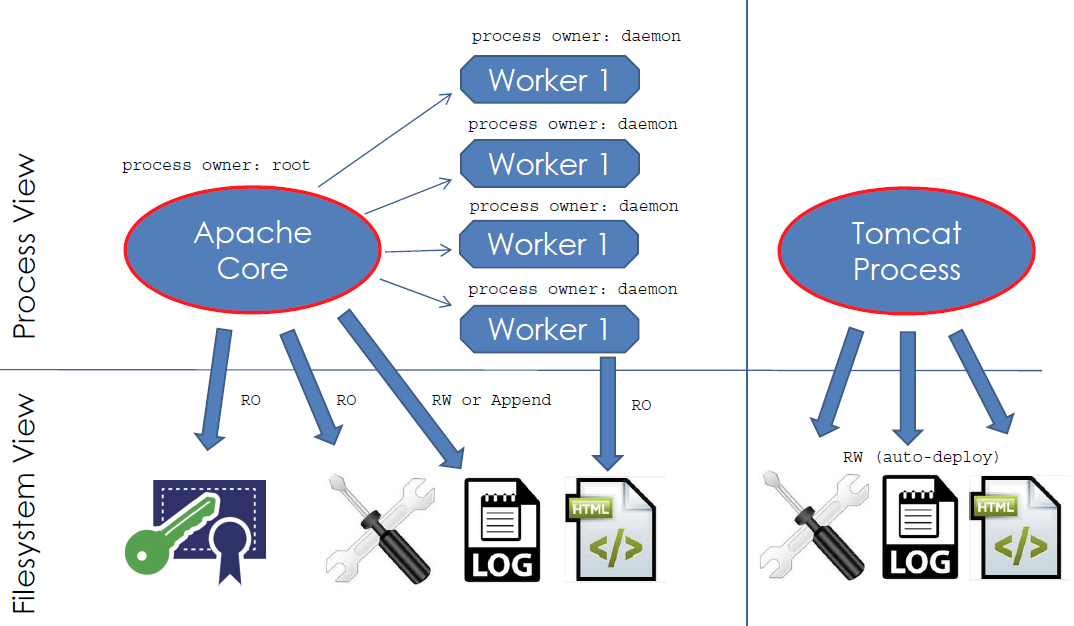
\includegraphics[width=\textwidth]{./img/apache_tomcat_permissions}
	\caption{Beispiel der Berechtigungen für Apache und Tomcat}
\end{figure}

\subsubsection{Apache File Permissions}
\begin{easylist}[itemize]
	& Im Besitz von Root
	&& Konfigurationsdateien
	&& SSL Schlüssel
	&& Log
	&& Html
	& Eigentümer des Apache Prozess benötigt nur RO
	&& Html
\end{easylist}

\subsubsection{Tomcat File Permissions}
Dies gestaltet sich oftmals schwierig, denn Tomcat besitzt eine andere Prozess-Architektur. Der Eigentümer des Tomcat-Prozess benötigt RW, für Remote Deployment, Konfiguration und Load Balancing.

\subsection{Privilege Escalation}
Dabei versteht man die Möglichkeit, die Berechtigungen des aktuellen Prozesses so zu verändern, dass man Zugriff auf andere geschützte Elemente erhält. Dazu können z.B. Bugs in SetUID-Tools verwendet werden.\\

Aber auch CRON kann gefährlich sein, da die Prozesse als Root gestartet werden. Wenn nun ein von CRON-Skript "'world-writeable"' ist, kann somit schnell etwas mit höchsten Berechtigungen ausgeführt werden.

\subsection{Network Hardening}
\textbf{Nur die nötigsten Dienste} sollten gegen Anfragen von aussen reagieren. Alle anderen müssen an \textit{localhost} gebunden sein. Alternativ kann auch eine \textbf{Firewall} dafür eingesetzt werden.\\
Dienste wie UPNP, Bonjour / Zeroconf und DLNA sollten aufgrund ihrer grossen Attach-Surface auch deaktiviert werden. Dies stammt daher, dass oftmals die Geräte unzureichende Authentifizierungsmechanismen implementiert haben.\\

Es wird in den Folien auch von der \textbf{Verwendung von IPv6 abgeraten}.\\

\textbf{ICMP-Redirects deaktivieren}, um MITM-Attacken vorzubeugen.\\

Eine Analyse mittels Nmap oder \fnurl{https://cisofy.com/lynis/}{Lynis von Cisofy} helfen, Schwachstellen aufzudecken.

\subsection{DB Hardening}
Wie auf das Dateisystem trifft das Prinzip Least Privileges auch auf die Datenbank zu. Der in der Anwendung hinterlegte Benutzer darf nur auf seine Datenbanken Berechtigungen erhalten. Es können in einer Anwendung auch mehrere Benutzer hinterlegt werden, mit unterschiedlichen Berechtigungen. So z.B. ein Benutzer nur mit \textit{SELECT}-Permissions für Abfragen, \textit{INSERT} und \textit{UPDATE} für Bestellungen und ein \textit{CREATE}, \textit{DELETE} für den DB-Admin.\\
\textbf{Keinesfalls sollte der Applikations-User \textit{GRANT}-Permissions erhalten.}

\include{_mobileappsecurity}

\section{Fraud Detection}
Fraud Detection beschreibt das Vorgehen um Betrugsfälle, wie zum Beispiel beim E-Banking, möglichst schnell zu erkennen und zu melden. Dabei wird der Computer als Hilfsmittel verwendet. Bis jetzt ist die Quote der gefundenen Fälle per Fraud Detection noch sehr gering. Weit über die Hälfte der Fälle werden durch Hinweise oder ein Management Review gefunden.

\subsection{Panopticlick / Client Correlator}
Panopticlick ist ein Softwareprojekt der Electronic Frontier Foundation (EFF). Das Konzept hinter der Software liegt darin, den Benutzer bei Besuch einer Webseite zu identifizieren, ohne dass dieser sich authentifizieren muss. Dafür wird ein Javascript auf dem Client ausgeführt, welches Informationen über den Browser sammelt. Daraus wird eine \textit{CCID} (Client Correlation ID) generiert. Diese wird auf dem Server mit bisherigen CCIDs verglichen. Somit kann man feststellen ob der Request von einem bereits bekannten Gerät kommt oder nicht. Um den Fingerprint des Browsers zu erstellen werden unter anderem folgende Daten einbezogen:
\begin{easylist}[itemize]
	& Verschlüsselte IP
	& Installierte Fonts
	& Installierte Plugins
	& Screen Resolution
	& Name des OS
	& User Agent String
\end{easylist}

\subsection{E-Banking}
E-Banking Systeme Verwenden zwei unterscheidliche Informationstypen um allfällige Frauds zu erkennen. Sollte bei der Überprüfung ein Verdacht auftauchen, kann die Transaktion gesperrt oder zum Beispiel per Telefon vom User bestätigt werden.

\subsubsection{Technische Daten}
Die Technischen Daten werden aus der Session gelesen. Die ausgelesenen Daten werden gegen alte gesammelte Daten verglichen.
Unter Anderem werden folgende Daten verwendet:
\begin{easylist}[itemize]
	& User Agent
	& Source IP
	& Zeit
	& Tippgeschwindigkeit
	& Durchschnittliche eingeloggte Zeit
\end{easylist}

\subsubsection{Business Informationen}
Bei den Business Informationen geht es um die getätigte Transaktion selber. Aufgrund dieser Daten könnte eine Fraud Transaction eventuell erkannt werden.
folgende Punkte werden untersucht:
\begin{easylist}[itemize]
	& Betrag
	& erstmalige Zahlung
	& An welche Bank geht die Zahlung (Inland / Ausland)
\end{easylist}

\subsection{Data Mining}
Data Mining beschreibt den Vorgang, um aus riesigen Mengen von Daten und Datensätzen, die wichtigen Informationen und zusammenhänge herauszufiltern.
Diese Fähigkeit, wichtige Informationen aus einer grossen Masse zu filtern, ist besonders für Vorhersagen oder Machine Learning interessant.
Durch Data Mining werden die Daten in Gruppen unterteilt.
Drei Common Tasks sind besonders nützlich für Fraud Detection:
\begin{easylist}[itemize]
	& Classification: Predictive, Kunden mit einer guten Kreditwürdigkeit suchen zum Beispiel
	& Clustering: Descriptive, Alle Kunden mit ähnlichem Einkaufsverhalten gruppieren
	& Association Rules: Artikel finden die oft mit dem gekauften zusammen gekauft werden
\end{easylist}

\subsection{Machine Learning}
Aufgrund der Informationen aus den Data Minings können Machine Learning Algorithmen eingesetzt werden, um zum Beispiel eine Transaktion als Verdächtig oder Harmlos einzustufen. Dies geschieht immer aufgrund bisher erhaltenen Transaktionen. Der Input (Neue Transaktion) wird also nacher als Richtwert für die nachfolgenden Transaktionen verwendet. So lernt der Automat dann von alleine. In der Vorlesung wurden verschiedene Algorithmen aufgezeigt:
\begin{easylist}[itemize]
	& Dempster–Shafer Theory
	& BLAST-SSAHA Hybridization
	& Hidden Markov Model
	& Evolutionary-fuzzy System
\end{easylist}

\subsection{Vorteile / Nachteile}
Die aufgezeigten Systeme können bereits automatisiert betrügerische Zahlungen erkennen und diese Melden, damit sie z.B. durch ein Mensch weiterverarbeitet werden. Je mehr Daten über den eigentlichen Benutzer zur verfügung stehen, umso besser funktioniert das ganze System. Ein automatisches System kann schneller reagieren und den Betrüger bereits stoppen, bevor ein Schaden entstanden ist.\\

Diese Fraud-Detection bringt jedoch viele Nachteile mit sich. Es ist es sehr aufwändig, ein solches System einzurichten und zu Betreiben. Damit sind grosse Kosten verbunden, denn es existieren kaum standardisierte Lösungen und auch keine ausgearbeiteten Konzepte. Zudem liefert es immer noch viele False Positives. Daher wird der Mensch wohl weiterhin eine zentrale Rolle spielen.

\include{_securitytesting}

\section{Spezialthemen}


\subsection{XXE File Inclusion}
Unter dem Begriff ist eine Attacke über das \textit{XML External Entity Processing} möglich. Dabei können externe Daten, wie z.B. lokale Dateien, in das XML inkludiert werden. Bei der Verarbeitung solcher Inclusions, welche im DTD angegeben sind, fügt sie der Parser in die angegebenen Stelle ein.\\

\textbf{Lösung:} Deaktivierung des Features für DTDs (External Entities) beim Parser.

\begin{lstlisting}[language=XML, caption=Beispiel der XXE]
<?xml version="1.0" encoding="ISO-8859-1"?>
<!DOCTYPE foo [  
  <!ELEMENT foo ANY >
  <!ENTITY xxe SYSTEM "file:///etc/passwd" >]>
<foo>&xxe;</foo>
\end{lstlisting}

\subsection{JSON-Hijacking}
JSON-Hijacking zielt darauf ab, sensitive Daten, die mittels JSON Format an einen authentifizierten Empfänger übermittelt werden, zu stehlen. Dabei präpariert der Angreifer eine Seite mit einem JavaScript, welches die Callback-Funktion oder den \textit{Property Setter} überschreibt. Als zweites wird ein GET Request auf die verwundbare Seite durchgeführt. Die Response kann dann vom Angreifer verarbeitet werden und die Daten (möglicherweise sensitive Informationen) auf seinem System speichern.\\

\textbf{Lösung:}
\begin{easylist}
	& Token in Request URLs verwenden, sodass diese nicht erraten werden können
	& JSON Response mit einem Infinite Loop beginnen
	& JSONP vermeiden
	& Arrays in ein JSON-Objekt einbetten
\end{easylist} 

\subsection{URL-Redirection}
URL-Redirection wird häufig im Zusammenhang mit Phishing verwendet, mit dem Ziel, eine Session übernehmen zu können. Dazu wird dem Opfer einen Link untergeschoben, der auf den ersten Blick vertrauenswürdig aussieht. In Wirklichkeit enthält dieser jedoch einen Redirect auf eine Landing-Page des Hackers. Klickt das Opfer auf diesen Link, so wird normal das Login-Formular der vertrauenswürdigen Webseite geladen. Gibt das Opfer nun seine Credentials ein, werden diese auf Korrektheit geprüft und es wird eine Session ausgestellt. Nach dem erfolgreichen Login, wird nun durch Redirection nicht die vertrauenswürdige Webseite geladen, sondern die Landing-Page des Hackers. Dadurch sieht der Hacker im Log seiner Page die ausgestellte Session und kann diese übernehmen. Das Opfer selbst erhält nur eine Meldung, dass die gewünschte Seite nicht erreichbar ist. \\

\textbf{Beispiel:} http://www.example.com/login?redirect=http://www.hack.er \\

\textbf{Lösung:}
\begin{easylist}
	& Inputvalidierung
	&& Parameter die Redirect URLS enthalten validieren
	&& Prüfen ob URL wirklich zur Seite gehört
	& Lookup Tables
	&& Erstellen von Mappings zwischen Parameter und URL
	&& redirect=1
	&& redirect=acc
\end{easylist} 

\subsection{HTTP Request Smuggling}
HTTP Request Smuggling Attacken werden benutzt, um beispielsweise WAFs zu umgehen. Dabei wird die Schwachstelle ausgenutzt, dass verschiedene Sicherheitssysteme HTTP Requests unterschiedlich interpretieren. Beispielsweise kann mit CR/LF (Carriage Return / Line Feed) erreicht werden, dass innerhalb eines einzigen Requests sich zwei Requests befinden. Die WAF erkennt nur den einen, der dahinter verborgene Webserver antwortet jedoch auf beide Requests. Somit können Informationen, die eigentlich nur zwischen WAF und Webserver sichtbar sein sollten, nach "'aussen"' gelangen. Beispielsweise ein Cookie welches zwischen WAF und Webserver einen User authentifiziert.\\

Oftmals werden die Felder Location und Set-Cookie als Ziel verwendet. Übliche Escape-Sequenzen sind: \lstinline|%0a %0d %0a%0d %0d%0a|

\begin{lstlisting}[language={},caption=Beispiel eines Präparierten Request zur Umgehung einer Pre-Authentication]
username=hacker10&url=%2Fsecure%0aSet-Cookie:LOGON=OK; %0aSet-Cookie:MOD_BUT_Username=admin;&lang=EN&password=compass
\end{lstlisting}

\textbf{Lösung:}
\begin{easylist}
	& Web Application Firewalls verwenden, die nicht verwundbar gegen HTTP Request Smuggling sind.
	& Strenges Sessionmanagement verwenden, z.B Session nach jedem Request terminieren.
	& Aktivieren von Strict Parsing beim Webserver, z.B. Apache.
\end{easylist} 

\subsection{Session Fixation}
Bei einer Session Fixation Attacke erzeugt der Hacker bei der verwundbaren Webseite eine Session (ohne Login). Diese Session wird nun dem Opfer mit einem Link mitgeteilt. Das Opfer authentifiziert sich auf der Webseite unter Verwendung dieser Session und ermöglicht es somit dem Hacker, die authentifizierte Session zu benützen.

\subsection{SSL/TLS: SSL-Cipher-Suite-Hardening, SSL-MitM}
\todo[inline]{SSL/TLS: SSL-Cipher-Suite-Hardening, SSL-MitM, muss noch ausgearbeitet werden}


\end{document}